\documentclass[12pt, a4paper]{article}
\usepackage[utf8]{inputenc}
\title{  Domača naloga\\\large\textbf{Simulacija spina v časovno odvisnem polju}\\
\large Računalniške tehnologije}
\usepackage{amsmath} 
\usepackage{braket}
\usepackage{listings}
\usepackage{graphicx}
\usepackage{float}
\usepackage{hyperref}
\author{Andrej Čop}
\date{Maj 2022}

\begin{document}
\maketitle
\newpage

\tableofcontents
\newpage

\section{Uvod}
V tej domači nalogi raziskujem dinamiko in precesijo spina v časovno spremenljivem polju. Najprej poiščem splošno rešitev za gibanje spina v polju v smeri $x$ in $z$. Nato dinamiko spina v časovno spremenljivem polju, kjer za nek čas $T$ deluje polje v $z$ smeri, nato pa za čas $bT$ deluje polje v smeri osi $x$. Napišem program v katerem simuliram pred tem opisano dinamiko po daljšem času in v odvisnosti od parametra $b$.

Celotna izvorna koda simulatorja in tudi tex od domače naloge se nahaja na repozitorju: \url{https://github.com/copandrej/Simulacija-spina} 
%komentar
\section{Izpeljava enačbe}
Po razdelku 3.75 iz učbenika \textit{Kvantne in računalniške tehnologije}, kjer je izpeljan Hamiltonov operator za elektronski spin v polju, lahko poiščemo splošno rešitev za gibanje spina če je magneto polje samo v smeri $x$ ali samo v smeri $z$.\\
Za smer $z$ je v učbeniku izpeljava že prikazana. Podobno naredimo v v smeri $x$:\\
\begin{equation}
H = \frac{h\omega}{2}
\begin{bmatrix}
0 & 1\\
1 & 0
\end{bmatrix}
\end{equation}\\
Lastni stanji sta kar $\ket{+}$ in $\ket{-}$ in časovnin razvoj je:


\begin{equation}
\ket{\psi(t)} = \cos\frac{\phi}{2}e^{-i(\phi+\omega_0 t)/2}\ket{+} + \sin\frac{\theta}{2}e^{i(\theta+\omega_0 t)/2}\ket{+}
\end{equation}\\
Kroženje(precesija) spina po \textit{Blochovi sferi}, imenovana tudi \textit{Larmorjeva precesija}, je tako podobna kot, če je polje v smeri $z$.

\section{Časovno odvisno polje}
Obravnavamo gibanje spina v časovno spremenljivem polju. S pomočjo programa, ki bo simuliral spin v kratkih časovnih intervalih in pri tem za čas $T$ uporabljamo enačbo za polje v smeri $z$ in nato za nek čas $bT$ v smeri $x$. 
\subparagraph{Hipoteza:}
Predvidevam, da za dovolj majhen $T$ in $b$ (tj. T precej manjši od obhodnega časa), bo rezultat simulacije precesija spina v obliki spirale na \textit{Blochovi sferi}

\section{Program za simuliranje}
Za simuliranje uporabljam programski jezik \textit{python} in module \textit{numpy, matplotlib}, \textit{cmath}, ter za simuliranje kvantnih sistemov in prikazovanje na Blochovi sferi \textit{qutip}.\\
Najprej nastavimo parametre in bazne vektorje:
\lstset{language=Python} 
\begin{lstlisting}
	t = 0.05
	T = math.pi
	time = theta = phi = 0
	frekvenca = 1 

	upSpin = basis(2, 0)
	downSpin = basis(2, 1)

	plus = (upSpin + downSpin)/math.sqrt(2)  # | + >
	minus = (upSpin - downSpin)/math.sqrt(2)  # | - >
\end{lstlisting}
Kljub večkratnim poiskusom nisem uspešno implementiral enačbe (2) v program, zato v nadaljevanju uporabljam koordinate Blochove sfere, ki jih izračunamo kot pričakovane vrednosti:
\begin{lstlisting}
	tocka = [cmath.sin(theta)*cmath.cos(phi), 
	cmath.sin(theta)*cmath.sin(phi), cmath.cos(theta)]
\end{lstlisting}
Koordinate periodično označujem na Blochovi sferi:
\begin{lstlisting}
	bl = qutip.Bloch()
	vektorji = []
		#v zanki	
		vektorji.append(tocka)
	bl.add_points(vektorji)
    	bl.render() 
\end{lstlisting}
Zanko poganjam na majhnih časovnih intervalih in pri tem posodabljam \textit{phi} in \textit{theta}: $\phi(t) = \phi + \omega_0t$
Med spreminjanjem smeri magnetnega polja posodobim kote $phi$ in $theta$ na zamenjana bazna vektorja z programom:
\begin{lstlisting}
	tocka[1] = 0
	norm = np.dot(tocka,tocka)
	tocka /= np.dot(tocka,tocka)
	dot_product = np.dot([1,0,0],tocka)
	theta = np.arccos(dot_product)
	phi = math.acos(norm)+math.pi 
\end{lstlisting}
\newpage
\section{Rezultati simulacije}
Primer simulacije precesije spina, ko je magnetno polje v smeri $z$ in kot $theta$ poljubno nastavljen:
\begin{figure}[H]
  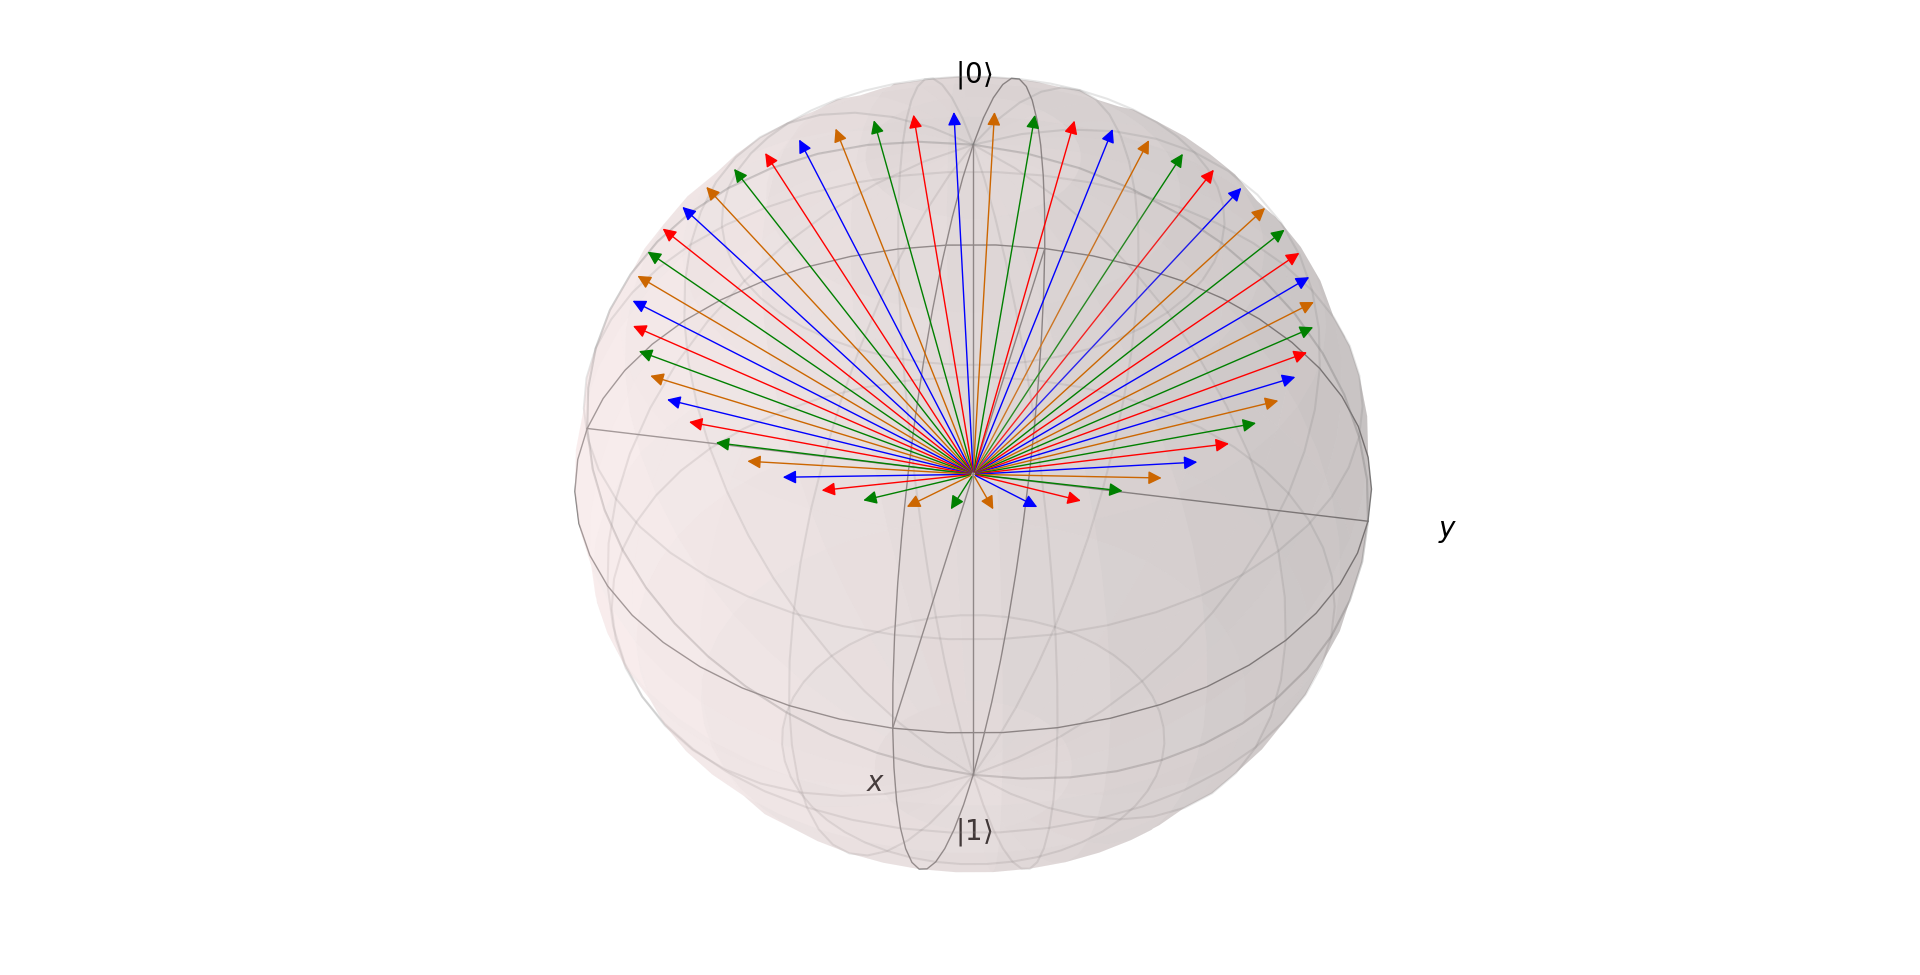
\includegraphics[width=500pt]{precesija_po_osi_z}
  \caption{Precesija spina, po magnetnem polju v smeri $z$}
  \label{fig:boat1}
\end{figure}
Primer simulacije pri časovno odvisnem polju, kot opisano v prejšnih razdelkih:
\section{Ugotovitve in zaključek}
Iz te simulacije lahko zaključimo, da se precesija spina podobno kot precesija vrtavke, z dodatno možnostjo časovno odvisnega magnetnega polja. Z spreminjanjem magnetnega polja in parametrov simulaciej lahko "pokrijemo" celotno Blochovo sfero.

Domača naloga je bila poučna predvsem iz smeri reševanja problemov in je pokazala, da zelo slabo pozanam ta področje, saj se je zalomilo že pri najbolj osnovnih izpeljavah in programiranju.

\section{Literatura}

\end{document}